\iffalse
\let\negmedspace\undefined
\let\negthickspace\undefined
\documentclass[journal,12pt,onecolumn]{IEEEtran}
\usepackage{cite}
\usepackage{amsmath,amssymb,amsfonts,amsthm}
\usepackage{algorithmic}
\usepackage{graphicx}
\usepackage{textcomp}
\usepackage{xcolor}
\usepackage{txfonts}
\usepackage{listings}
\usepackage{enumitem}
\usepackage{mathtools}
\usepackage{gensymb}
\usepackage[breaklinks=true]{hyperref}
\usepackage{tkz-euclide} % loads  TikZ and tkz-base
\usepackage{listings}
\usepackage{float}
\newtheorem{theorem}{Theorem}[section]
\newtheorem{problem}{Problem}
\newtheorem{proposition}{Proposition}[section]
\newtheorem{lemma}{Lemma}[section]
\newtheorem{corollary}[theorem]{Corollary}
\newtheorem{example}{Example}[section]
\newtheorem{definition}[problem]{Definition}
\newcommand{\BEQA}{\begin{eqnarray}}
\newcommand{\EEQA}{\end{eqnarray}}
\newcommand{\define}{\stackrel{\triangle}{=}}
\theoremstyle{remark}
\newtheorem{rem}{Remark}
\parindent 0px

\begin{document}
%
\providecommand{\pr}[1]{\ensuremath{\Pr\left(#1\right)}}
\providecommand{\prt}[2]{\ensuremath{p_{#1}^{\left(#2\right)} }}        % own macro for this question
\providecommand{\qfunc}[1]{\ensuremath{Q\left(#1\right)}}
\providecommand{\sbrak}[1]{\ensuremath{{}\left[#1\right]}}
\providecommand{\lsbrak}[1]{\ensuremath{{}\left[#1\right.}}
\providecommand{\rsbrak}[1]{\ensuremath{{}\left.#1\right]}}
\providecommand{\brak}[1]{\ensuremath{\left(#1\right)}}
\providecommand{\lbrak}[1]{\ensuremath{\left(#1\right.}}
\providecommand{\rbrak}[1]{\ensuremath{\left.#1\right)}}
\providecommand{\cbrak}[1]{\ensuremath{\left\{#1\right\}}}
\providecommand{\lcbrak}[1]{\ensuremath{\left\{#1\right.}}
\providecommand{\rcbrak}[1]{\ensuremath{\left.#1\right\}}}
\newcommand{\sgn}{\mathop{\mathrm{sgn}}}
\providecommand{\abs}[1]{\left\vert#1\right\vert}
\providecommand{\res}[1]{\Res\displaylimits_{#1}} 
\providecommand{\norm}[1]{\left\lVert#1\right\rVert}
%\providecommand{\norm}[1]{\lVert#1\rVert}
\providecommand{\mtx}[1]{\mathbf{#1}}
\providecommand{\mean}[1]{E\left[ #1 \right]}
\providecommand{\cond}[2]{#1\middle|#2}
\providecommand{\fourier}{\overset{\mathcal{F}}{ \rightleftharpoons}}
\newenvironment{amatrix}[1]{%
  \left(\begin{array}{@{}*{#1}{c}|c@{}}
}{%
  \end{array}\right)
}
\newcommand{\solution}{\noindent \textbf{Solution: }}
\newcommand{\cosec}{\,\text{cosec}\,}
\providecommand{\dec}[2]{\ensuremath{\overset{#1}{\underset{#2}{\gtrless}}}}
\newcommand{\myvec}[1]{\ensuremath{\begin{pmatrix}#1\end{pmatrix}}}
\newcommand{\mydet}[1]{\ensuremath{\begin{vmatrix}#1\end{vmatrix}}}
\newcommand{\myaugvec}[2]{\ensuremath{\begin{amatrix}{#1}#2\end{amatrix}}}
\providecommand{\rank}{\text{rank}}
\providecommand{\pr}[1]{\ensuremath{\Pr\left(#1\right)}}
\providecommand{\qfunc}[1]{\ensuremath{Q\left(#1\right)}}
	\newcommand*{\permcomb}[4][0mu]{{{}^{#3}\mkern#1#2_{#4}}}
\newcommand*{\perm}[1][-3mu]{\permcomb[#1]{P}}
\newcommand*{\comb}[1][-1mu]{\permcomb[#1]{C}}
\providecommand{\qfunc}[1]{\ensuremath{Q\left(#1\right)}}

\providecommand{\gauss}[2]{\mathcal{N}\ensuremath{\left(#1,#2\right)}}
\providecommand{\diff}[2]{\ensuremath{\frac{d{#1}}{d{#2}}}}
\providecommand{\myceil}[1]{\left \lceil #1 \right \rceil }
\newcommand\figref{Fig.~\ref}
\newcommand\tabref{Table~\ref}
\newcommand{\sinc}{\,\text{sinc}\,}
\newcommand{\rect}{\,\text{rect}\,}
\let\StandardTheFigure\thefigure
\let\vec\mathbf


\bibliographystyle{IEEEtran}


\vspace{3cm}

\title{
%	\logo{
Q-9.3.30
%	}
}
\author{Snehil Singh - EE22BTECH11050}


\maketitle
\textbf{Question:} The probability of guessing correctly at least 8 out of 10 answers on a true-false type
examination is
\solution
\fi
Defining variables:
\begin{table}[H]
\def\arraystretch{1.2}
\begin{tabular}{|c|c|c|}
\hline
	\textbf{Parameter} &\textbf{Value} &\textbf{Description}\\ \hline
	$n$ &10 &Number of questions\\ 
	\hline
	$p$ &0.5 & probability of guessing correctly\\ 
	\hline
	$\mu = np$ &5 & mean of the distribution\\ 
	\hline
	$\sigma^2 = np(1-p)$ &2.5 & variance of the distribution\\ 
	\hline
	$Y$ & 0-10 & denotes number of questions guessed correctly\\
	\hline
\end{tabular}
\end{table}
\begin{enumerate}
\item \textbf{Binomial distribution:} 
the probability of getting exactly 8 correct answers is 
\begin{align}
	&= \binom{10}{8} \times 0.5^8\times 0.5^{2}\\
	&= 0.043946
\end{align}
\item \textbf{Gaussian Distribution:}\\
The gaussian distribution for $Y$ is
\begin{align}
	p_Y(x) = \frac{1}{\sqrt{2\pi\sigma^2}}e^{\frac{-(x-\mu)^2}{2\sigma^2}}\label{9.3.30}
\end{align}
For getting exactly 8 correct answers
\begin{align}
	Y &= 8
\end{align}
Substituting in equation \eqref{9.3.31}, probability for getting exactly 8 correct answers is
\begin{align}
	p_Y(8) &= \frac{1}{\sqrt{2\pi\times2.5}}e^{\frac{-(8-5)^2}{2\times2.5}}\\
	&= 0.05204
\end{align}
\begin{figure}[H]
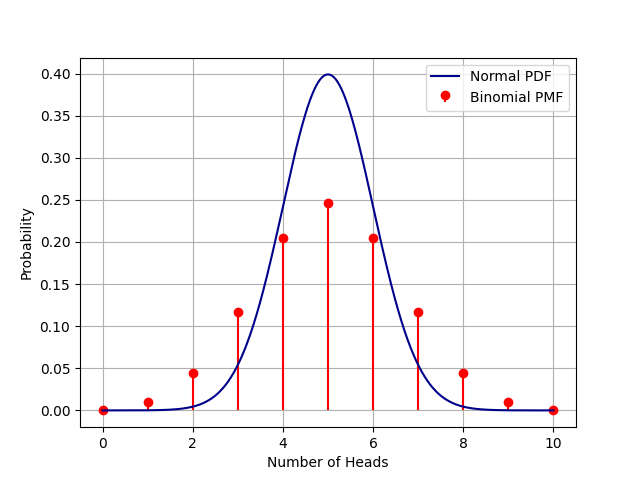
\includegraphics[width=\columnwidth]{ncert/9/3/30/figs/fig.png}
\caption{Binomial distribution vs Gaussian distribution}
	\label{fig58:_9_3_30}
\end{figure}
\item \textbf{Using Q function:}
Defining a gaussian random variable Z such that
\begin{align}
	Z \sim \gauss{\mu}{\sigma^2}
\end{align}
Due to continuity correction, $\Pr(Z=x)$ can be approximated as
\begin{align}
	p_Z(x) &\approx \Pr(x-0.5\le Z < x+0.5)\\
	&\approx \Pr(Z < x+0.5) - \Pr(Z < x-0.5)\\
	&\approx F_Z(x+0.5)-F_Z(x-0.5)
\end{align}
CDF of Z is defined as -
\begin{align}
	F_Z(x) &= \Pr(Z<x)\\
	&= \Pr\biggl(\frac{Z-\mu}{\sigma}<\frac{x-\mu}{\sigma}\biggr)
\end{align}
As
\begin{align}
	\frac{Z-\mu}{\sigma} &\sim \gauss{0}{1}\\
	\implies F_Z(x) 
	&= 1 - \Pr\biggl(\frac{Z-\mu}{\sigma}>\frac{x-\mu}{\sigma}\biggr)\\
	&= \begin{cases}
		1-Q(\frac{x-\mu}{\sigma}) & x\geq \mu\\
		Q(\frac{\mu-x}{\sigma}) & x < \mu
	\end{cases}
\end{align}
$\therefore$ Gaussian approximation for $\Pr(Z = 8)$ is 
\begin{align}
	p_Z(8) &= 1-Q(1.63273) \\
	&= 0.051263
\end{align}
\end{enumerate}



